% !TeX program = xelatex
\documentclass{ctexart}
\usepackage[table]{xcolor}
\usepackage{template_by_mny}
\usepackage{float} 
\usepackage{listings}
\lstset{basicstyle=\ttfamily, breaklines=true, frame=single}

\title{光谱仪教学实验报告}
\class{物理 32/物理 31}
\name{冯家琦/周方远}
\id{2023011338/2023011263}

\begin{document}
\maketitle

\begin{abstract}
本实验使用EDU-SPEB2光谱仪教学套件,完成了入射狭缝宽度对光谱分辨率的影响、LED光谱观测以及汞光谱中三条谱线波长测量等实验。通过实验加深了对光谱仪工作原理的理解,掌握了光谱测量的基本方法。
\end{abstract}

\section{实验原理}

光谱仪是一种用于分析光谱的光学仪器。其基本原理包括:

\subsection{三棱镜折射}
* 三棱镜折射角公式:

\subsection{光谱仪的组成}
一个基本的光谱仪包含以下部件:
\begin{itemize}
    \item 入射狭缝:控制入射光束宽度
    \item 准直系统:将发散光束准直
    \item 分光元件:三棱镜
    \item 聚焦系统:将分光后的光聚焦
    \item 观测屏/探测器:用于观测光谱
\end{itemize}

\section{实验仪器及安装}
\subsection{实验仪器}
\begin{itemize}
    \item EDU-SPEB2光谱仪教学套件
    \item 可调节狭缝
    \item 三棱镜
    \item LED光源及其USB供电支架
    \item 双凸透镜(f=50mm和100mm)
    \item 观测屏
    \item 其他光学元件支架和固定件
\end{itemize}
\subsection{仪器安装}
\subsubsection{光源安装}
先在左侧固定光源,再在光源后 24cm 处固定可调节狭缝,并确保两者在同一光路中。

在光源与可调狭缝正中间放置 50mm 透镜,然后将透镜缓慢向光源移动直到可调狭缝上出现清晰的像。调好后将透镜固定。
\begin{figure}[htbp]
    \centering
    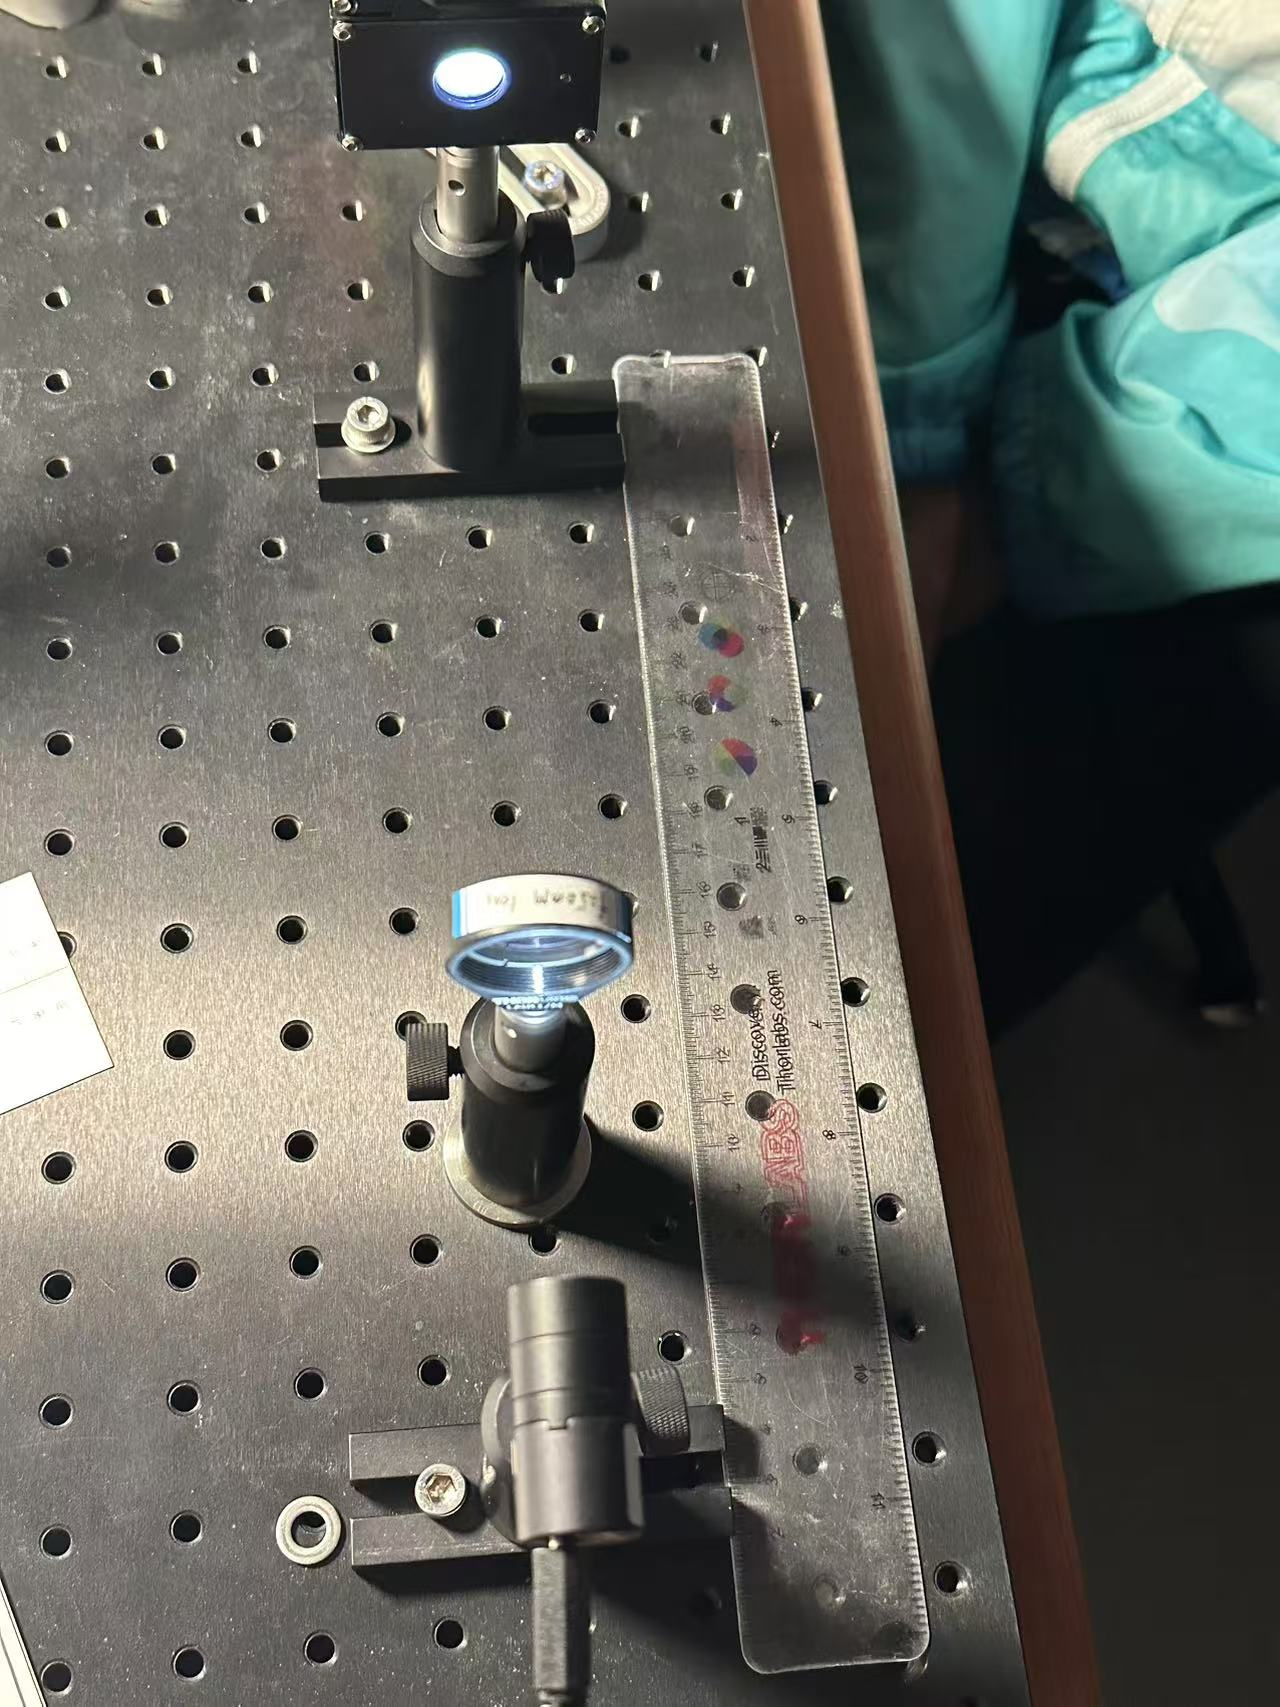
\includegraphics[width=0.2\textwidth,height=0.3\textwidth]{pictures/微信图片_20241107162037.jpg}
    \caption{LED光源安装}
\end{figure}
\subsubsection{三棱镜光谱仪安装}
*
\section{实验步骤}

\subsection{实验一:LED光谱观测}
**
1. 将LED安装在USB供电支架上并通电。LED的光谱如图,可以看到有两个尖峰,并且在蓝色和绿色之间波长的光非常弱,几乎消失。
\begin{figure}[H]
    \centering
    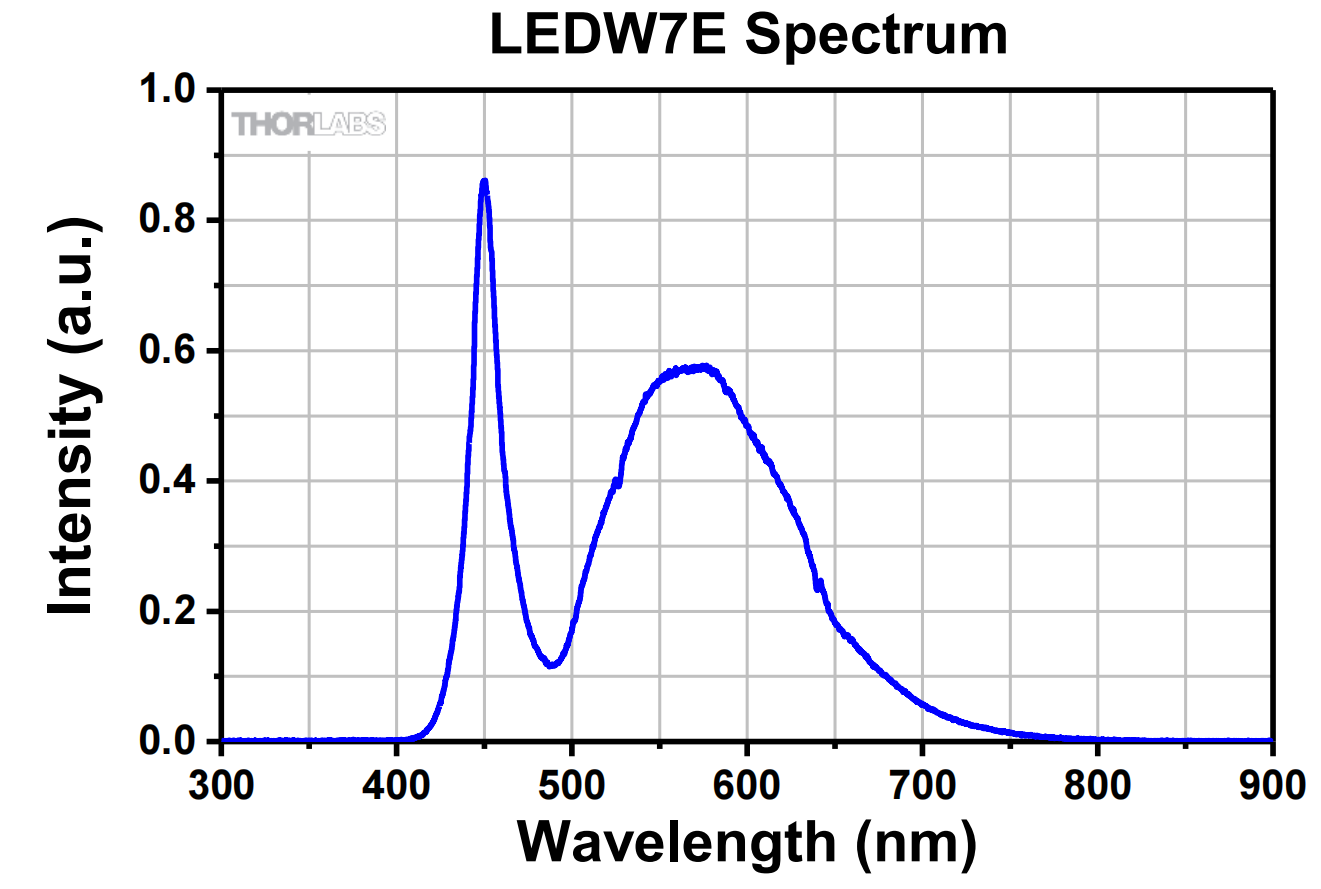
\includegraphics[width=0.4\textwidth,height=0.2\textwidth]{pictures/光谱图.png}
    \caption{LED理论光谱}
\end{figure}

2. 经过观察如图
\begin{figure}[H]
    \centering
    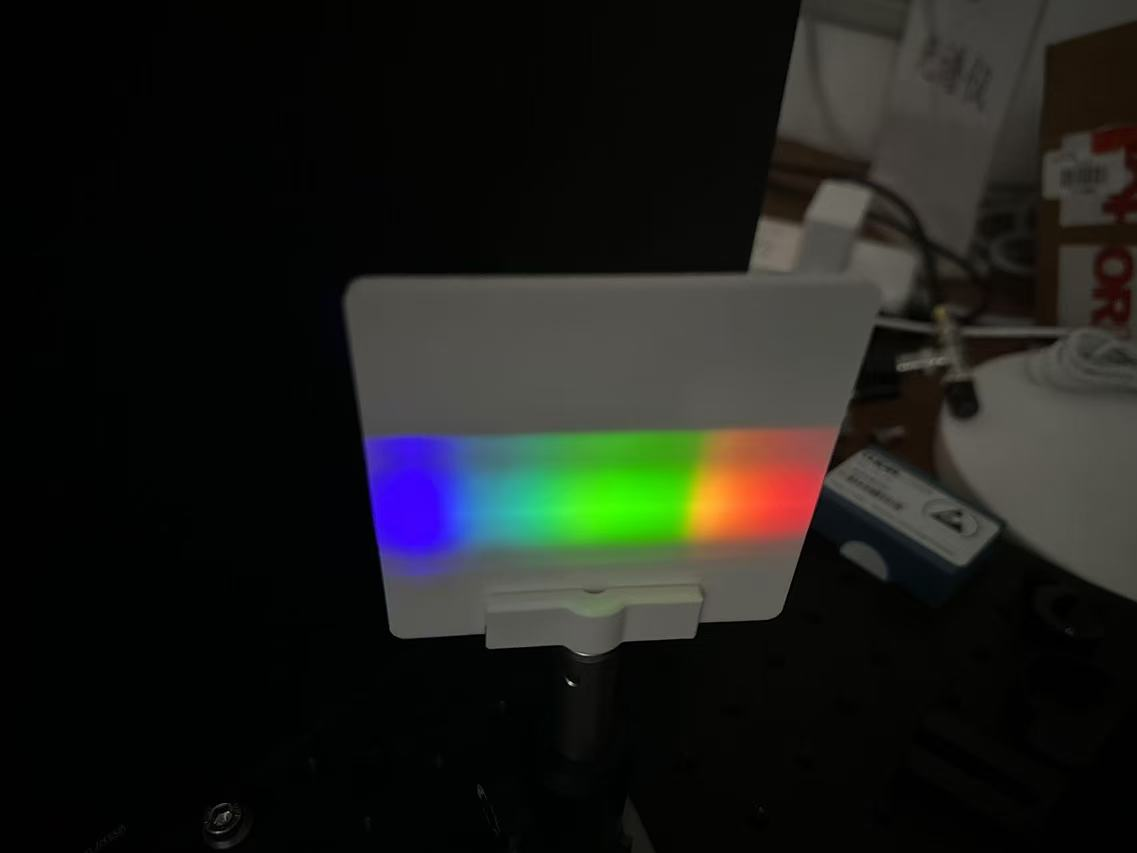
\includegraphics[width=0.4\textwidth,height=0.2\textwidth]{pictures/微信图片_20241107162045.jpg}
    \caption{LED观察光谱}
\end{figure}
与理论相符,可以看到蓝色和绿色之间的光强非常弱。

\subsection{实验二:已知光谱线的棱镜折射率测量}
**

\section{实验思考}

\subsection{LED光谱特征}
LED发出的是连续光谱,但在特定波长范围内强度较大。这反映了LED的发光机理是由电子在半导体能带间跃迁产生的。

\subsection{三棱镜光谱测量}
**

\section{总结}

通过本次实验,我们:
\begin{itemize}
    \item 理解了光谱仪的基本工作原理
    \item 掌握了调节光谱仪的方法
    \item 学会了测量三棱镜的折射率
    \item 认识到了不同光源的光谱特征
\end{itemize}

实验过程中发现光路调节较为关键,需要仔细进行准直和聚焦。建议在后续实验中可以增加不同光源的对比分析。

\end{document}